\documentclass{article}
\usepackage{amssymb}
\usepackage{graphicx}
%Week 1
\begin{document}

\section{Signals}
Signals are defined to be a function that conveys information about a phenomenon.
They can also be said to be a medium which carry information relevant to a reciever.

Electromagnetic wave, voltage or current carrying information are some examples of signals.

\subsection{Are there any non-time based signals?}
\begin{itemize}
    \item Images: They are represented as a combination of  monochrome images in three primary colors.
    $$ Image: \mathbb{R}^2 \rightarrow \{ R, G, B\}$$
    \item Temperature at various points in a room.
    $$ Temperature:\mathbb{R}^3 \rightarrow K \quad(or\; Celsius)$$
    \item Videos:  A video signal is a sequence of images.
    \item Text or a page in a book.
\end{itemize}

\section{Communication}
Communication is the process of exchanging information. Transmission, reception and reconstruction of the transmitted signal take place in this process.
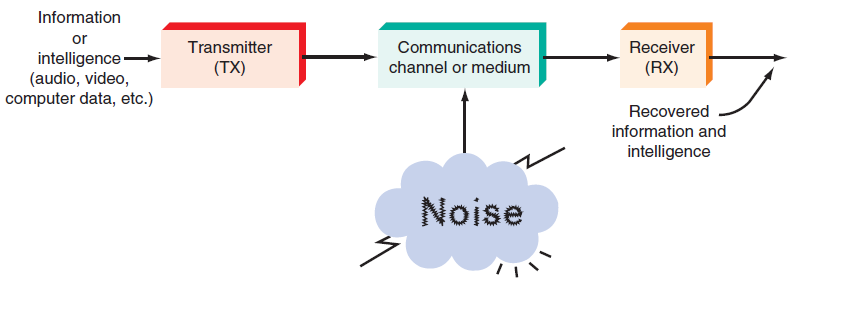
\includegraphics[width=\textwidth]{ptp.png}

Channel: Separates the source and reciever and is not directly under our control.
This leads to some disturbances or imperfections in the channel, which is called noise.



\end{document}
